% A LaTeX template for MSc Thesis submissions to 
% Politecnico di Milano (PoliMi) - School of Industrial and Information Engineering
%
% S. Bonetti, A. Gruttadauria, G. Mescolini, A. Zingaro
% e-mail: template-tesi-ingind@polimi.it
%
% Last Revision: October 2021
%
% Copyright 2021 Politecnico di Milano, Italy. NC-BY

\documentclass{Configuration_Files/PoliMi3i_thesis}
%------------------------------------------------------------------------------
%	REQUIRED PACKAGES AND  CONFIGURATIONS
%------------------------------------------------------------------------------

% CONFIGURATIONS
\usepackage{rotating, caption}
\usepackage{pdflscape}
\usepackage{pdfpages}
\usepackage{minted}
\usepackage{comment}
\usepackage{listings}
\usepackage{parskip} % For paragraph layout
\usepackage{setspace} % For using single or double spacing
\usepackage{emptypage} % To insert empty pages
\usepackage{multicol} % To write in multiple columns (executive summary)
\setlength\columnsep{15pt} % Column separation in executive summary
\setlength\parindent{0pt} % Indentation
\raggedbottom  

% PACKAGES FOR TITLES
\usepackage{titlesec}
% \titlespacing{\section}{left spacing}{before spacing}{after spacing}
\titlespacing{\section}{0pt}{3.3ex}{2ex}
\titlespacing{\subsection}{0pt}{3.3ex}{1.65ex}
\titlespacing{\subsubsection}{0pt}{3.3ex}{1ex}
\usepackage{color}

% PACKAGES FOR LANGUAGE AND FONT
\usepackage[english]{babel} % The document is in English  
\usepackage[utf8x]{inputenc} % UTF8 encoding
\usepackage[T1]{fontenc} % Font encoding
\usepackage[11pt]{moresize} % Big fonts

% PACKAGES FOR IMAGES
\usepackage{graphicx}
\usepackage{transparent} % Enables transparent images
\usepackage{eso-pic} % For the background picture on the title page
\usepackage{subfig} % Numbered and caption subfigures using \subfloat.
\usepackage{tikz} % A package for high-quality hand-made figures.
\usetikzlibrary{}
\graphicspath{{./Images/}} % Directory of the images
\usepackage{caption} % Coloured captions
\usepackage{xcolor} % Coloured captions
\usepackage{amsthm,thmtools,xcolor} % Coloured "Theorem"
\usepackage{float}
\usepackage{wrapfig}

% STANDARD MATH PACKAGES
\usepackage{amsmath}
\usepackage{amsthm}
\usepackage{amssymb}
\usepackage{amsfonts}
\usepackage{bm}
\usepackage[overload]{empheq} % For braced-style systems of equations.
\usepackage{fix-cm} % To override original LaTeX restrictions on sizes

% PACKAGES FOR TABLES
\usepackage{tabularx}
\usepackage{longtable} % Tables that can span several pages
\usepackage{colortbl}
\usepackage{multirow}
\usepackage{longtable}
% PACKAGES FOR ALGORITHMS (PSEUDO-CODE)
\usepackage{algorithm}
\usepackage{algorithmic}
\usepackage{blindtext}


\usepackage[absolute]{textpos}
\usepackage{fancyhdr}
\fancypagestyle{lscape}{% 
\fancyhf{} % clear all header and footer fields 
\fancyfoot[LE]{%
\begin{textblock}{20}(1,5){\rotatebox{90}{\leftmark}}\end{textblock}
\begin{textblock}{1}(13,10.5){\rotatebox{90}{\thepage}}\end{textblock}}
\fancyfoot[LO] {%
\begin{textblock}{1}(13,10.5){\rotatebox{90}{\thepage}}\end{textblock}
\begin{textblock}{20}(1,13.25){\rotatebox{90}{\rightmark}}\end{textblock}}
\renewcommand{\headrulewidth}{0pt} 
\renewcommand{\footrulewidth}{0pt}}


% PACKAGES FOR REFERENCES & BIBLIOGRAPHY
%\usepackage[colorlinks=true,linkcolor=black,anchorcolor=black,citecolor=black,filecolor=black,menucolor=black,runcolor=black,urlcolor=black]{hyperref} % Adds clickable links at references
%\usepackage{cleveref}
%\usepackage[square, numbers, sort&compress]{natbib} % Square brackets, citing references with numbers, citations sorted by appearance in the text and compressed
%\bibliographystyle{siam} % You may use a different style adapted to your field

% PACKAGES FOR REFERENCES & BIBLIOGRAPHY
\usepackage[colorlinks=true,linkcolor=black,anchorcolor=black,citecolor=black,filecolor=black,menucolor=black,runcolor=black,urlcolor=black]{hyperref} % Adds clickable links at references
\usepackage{cleveref}
\usepackage[square, numbers, sort&compress]{natbib} % Square brackets, citing references with numbers, citations sorted by appearance in the text and compressed
\bibliographystyle{abbrvnat} % You may use a different style adapted to your field


% OTHER PACKAGES
\usepackage{pdfpages} % To include a pdf file
\usepackage{afterpage}
\usepackage{lipsum} % DUMMY PACKAGE
\usepackage{fancyhdr} % For the headers
\fancyhf{}
\usepackage{eurosym}

% Input of configuration file. Do not change config.tex file unless you really know what you are doing. 
% Define blue color typical of polimi
\definecolor{bluepoli}{cmyk}{0.4,0.1,0,0.4}

% Custom theorem environments
\declaretheoremstyle[
  headfont=\color{bluepoli}\normalfont\bfseries,
  bodyfont=\color{black}\normalfont\itshape,
]{colored}

% Set-up caption colors
\captionsetup[figure]{labelfont={color=bluepoli}} % Set colour of the captions
\captionsetup[table]{labelfont={color=bluepoli}} % Set colour of the captions
%\captionsetup[algorithm]{labelfont={color=bluepoli}} % Set colour of the captions

\theoremstyle{colored}
\newtheorem{theorem}{Theorem}[chapter]
\newtheorem{proposition}{Proposition}[chapter]

% Enhances the features of the standard "table" and "tabular" environments.
\newcommand\T{\rule{0pt}{2.6ex}}
\newcommand\B{\rule[-1.2ex]{0pt}{0pt}}

% Pseudo-code algorithm descriptions.
%\newcounter{algsubstate}
%\renewcommand{\thealgsubstate}{\alph{algsubstate}}
%\newenvironment{algsubstates}
 % {\setcounter{algsubstate}{0}%
  % \renewcommand{\STATE}{%
   %  \stepcounter{algsubstate}%
    % \Statex {\small\thealgsubstate:}\space}}
  %{}

% New font size
\newcommand\numfontsize{\@setfontsize\Huge{200}{60}}

% Title format: chapter
\titleformat{\chapter}[hang]{
\fontsize{50}{20}\selectfont\bfseries\filright}{\textcolor{bluepoli} \thechapter\hsp\hspace{2mm}\textcolor{bluepoli}{|   }\hsp}{0pt}{\huge\bfseries \textcolor{bluepoli}
}

% Title format: section
\titleformat{\section}
{\color{bluepoli}\normalfont\Large\bfseries}
{\color{bluepoli}\thesection.}{1em}{}

% Title format: subsection
\titleformat{\subsection}
{\color{bluepoli}\normalfont\large\bfseries}
{\color{bluepoli}\thesubsection.}{1em}{}

% Title format: subsubsection
\titleformat{\subsubsection}
{\color{bluepoli}\normalfont\large\bfseries}
{\color{bluepoli}\thesubsubsection.}{1em}{}

% Shortening for setting no horizontal-spacing
\newcommand{\hsp}{\hspace{0pt}}

\makeatletter
% Renewcommand: cleardoublepage including the background pic
\renewcommand*\cleardoublepage{%
  \clearpage\if@twoside\ifodd\c@page\else
  \null
  \AddToShipoutPicture*{\BackgroundPic}
  \thispagestyle{empty}%
  \newpage
  \if@twocolumn\hbox{}\newpage\fi\fi\fi}
\makeatother

%For correctly numbering algorithms
%\numberwithin{algorithm}{chapter}

%----------------------------------------------------------------------------
%	NEW COMMANDS DEFINED
%----------------------------------------------------------------------------

% EXAMPLES OF NEW COMMANDS
\newcommand{\bea}{\begin{eqnarray}} % Shortcut for equation arrays
\newcommand{\eea}{\end{eqnarray}}
\newcommand{\e}[1]{\times 10^{#1}}  % Powers of 10 notation

%----------------------------------------------------------------------------
%	ADD YOUR PACKAGES (be careful of package interaction)
%----------------------------------------------------------------------------
%\usepackage{pgfplots}
\usepackage{lscape}
\usepackage{rotating}
\usepackage{lipsum}


%----------------------------------------------------------------------------
%	ADD YOUR DEFINITIONS AND COMMANDS (be careful of existing commands)
%----------------------------------------------------------------------------
\newsavebox{\mybox}
%----------------------------------------------------------------------------
%	BEGIN OF YOUR DOCUMENT
%----------------------------------------------------------------------------




\begin{document}


\fancypagestyle{plain}{%
\fancyhf{} % Clear all header and footer fields
\fancyhead[RO,RE]{\thepage} %RO=right odd, RE=right even
\renewcommand{\headrulewidth}{0pt}
\renewcommand{\footrulewidth}{0pt}}

%----------------------------------------------------------------------------
%	TITLE PAGE
%----------------------------------------------------------------------------

\pagestyle{empty} % No page numbers
\frontmatter % Use roman page numbering style (i, ii, iii, iv...) for the preamble pages

\puttitle{
	title=Controlling management systems applied to LPT Italian companies, % Title of the thesis
	name= \\ 
	      \vspace{0.2 cm}\\
	      Chiara Beretta \hspace{2,2 cm} 10615536 \\ 
          \vspace{0.01 cm}  \\   
          Seyed Hesam Babaei \hspace{0,99 cm} 10780315 \\ 
          \vspace{0.01 cm}\\ 
          Luca Cattaneo \hspace{2,2 cm} 10521219 \\ 
          \vspace{0.01 cm}\\          
          Pietro Mariano \hspace{2,1 cm} 10529938 \\
          \vspace{0.01 cm}\\
          Fabio Vitiello \hspace{2,5 cm} 10529938, % Author Name and Surname
	course= MOBILITY: INFRASTRUCTURES AND SERVICES , % Study Programme (in Italian)
	academicyear={2021-2022},  % Academic Year
} % These info will be put into your Title page 

%----------------------------------------------------------------------------
%	PREAMBLE PAGES: ABSTRACT (inglese e italiano), EXECUTIVE SUMMARY
%----------------------------------------------------------------------------
\startpreamble
\setcounter{page}{1} % Set page counter to 1

% ABSTRACT IN ENGLISH

\include{Chapters/00_Abstract}

%----------------------------------------------------------------------------
%	LIST OF CONTENTS/FIGURES/TABLES/SYMBOLS
%----------------------------------------------------------------------------

% TABLE OF CONTENTS
\thispagestyle{empty}
\tableofcontents % Table of contents 
\thispagestyle{empty}
\cleardoublepage

%-------------------------------------------------------------------------
%	THESIS MAIN TEXT
%-------------------------------------------------------------------------
% In the main text of your thesis you can write the chapters in two different ways:
%
%(1) As presented in this template you can write:
%    \chapter{Title of the chapter}
%    *body of the chapter*
%
%(2) You can write your chapter in a separated .tex file and then include it in the main file with the following command:
%    \chapter{Title of the chapter}
%    \input{chapter_file.tex}
%
% Especially for long thesis, we recommend you the second option.

%\addtocontents{toc}{\vspace{2em}} % Add a gap in the Contents, for aesthetics
\mainmatter % Begin numeric (1,2,3...) page numbering
% --------------------------------------------------------------------------
% NUMBERED CHAPTERS % Regular chapters following
% --------------------------------------------------------------------------
\chapter{Introduction}




















\chapter{State of the Art}

\paragraph{What is Arriva}
Arriva Italia is the Arriva Group’s italian branch. Present on the Italian market since 2002, managing around $5\%$ of the market shares, it provides both urban and extra-urban transport services mainly in Northern Italy, as well as shuttle services to Turin and Milan airports.

With respect to our case study Arriva Italia is member of the Bergamo trasporti consortium from the 2002 with the acquisition of \emph{SAB autoservizi} and directly from 2020 with the incorporation of SAB.

\subparagraph{The consortium}
The Consortium is an association of different companies built in 2003 for the tender about the Subnetwork SUD of the Province of Bergamo.
The different companies that are part of the consortium are: SAI Società Autolinee Interprovinciali srl, Arriva Italia srl, AGI Auto Guidovie Italiane SpA, Autoservizi Locatelli srl, TBSO Trasporti Bergamo Sud Ovest SpA e Autoservizi Zani srl.

\paragraph{What is a dashboard}
As reported on the official website of Microsoft a dashboard is a tool to track, analyze and display data about a process or an organization to obtain insight.

The benefits are different such as performance measure, data transparency and forecasting.


\subparagraph{Apllication on the LPT}

In our study case the dashboard can be a useful instrument to allow both the PTO and PTA check the respect of the requirements provided from the contract of service. Then the PTO can define useful relation between the KPIs themselves. 

So, to start our analysis the Service contract must be read and analyzed.
\section{Analysis of Contract of Service}
%Analysis of the contract of service. From that  the defined KPI  to put in "traditional dashboard"
\paragraph{What is a service contract?}
%explain what is the service contract and some background in the context
The service contract regulates the discharge of a public service by an operator as decided by the public autorithy. In case of public transport the autorithy is call PTA and the operator PTO. The service contract are generally made after a tender and are regulated by the REGULATION (EC) No 1370/2007 at european level and by the italian legislative decree No 422/2007 that respeclty define the norms about the public transport service on road and rails and assign the function to the different italian local entities.

\paragraph{Our study case: Bergamo Trasporti Consortium}
The study case is about the public transport service of the subnetwork sud of the province of Bergamo (with the Province of Bergamo as PTA) and the Bergamo trasporti consortium as PTO.

\subparagraph{History of the service} The service has started in 2005 of the service after the winning of the tender by the consurtion in 2004. Then a first extension has been made in 2011 (the natural expiration year) until 2014 without changes in the requirements. Then another extension has been made with changes in the contract of service in particular:
\begin{itemize}
    \item the required number of $bus-km\cdot year$ rised up to $4345000$
    \item the grants
    \item the bus fleet
\end{itemize}

Then in 2019 the PTA use the power provided by the article 5 of REGULATION (EC) No 1370/2007 and use the \emph{requriment to provide} to extend the duration of the contract of service until 31/12/2021. This act also change the previous requirements/conditions:
\begin{itemize}
    \item 4.240.000 vetture-km
\end{itemize}

\subparagraph{Effects of COVID-19 in the contract of service}
Due to the COVID-19 emergency the PTA and PTO make a change in the contract of service in particular in the authorization of changes in service due to COVID prevention measure (example school closure) and the change of the bus fleet requirements with an increase of the maximum age of the bus from 15 years to 18 years without restriction and allow the bus with a maxium age of 21 years if the not exced the maxium of 1 milion km.

Then in 2021 with the last requirement ot provide the service has been extended until 2023.

\subparagraph{KPIs from the Contract of Service}
From the contract of service can be directly obtained the following KPIs\footnote{For better visualizing the trend a focus on the last requirement to provide has been made to have a more actual legislative situation}:
\begin{itemize}
    \item Bus fleet requirements:
    \begin{itemize}
        \item Age of the fleet (the last requirement to provide put a maximum of 18 years and 22 year 21 with restrinctions)
        \item If it is climatezed (all the fleet must be climatized)
        \item The emissions regulation (EU6, EU5, EU4, ...).
        \item the accessibility for people no autosufficiently
    \end{itemize}
    \item suppressed lines with the distiction by lines, years and companies
\end{itemize}


\chapter{Traditional dashboard}
%The dashboard created on PowerBI 
From the KPIs founded in the analysis of the contract we decide to visualize them by creating an off-line dashboard with PowerBi to find other useful information that without visualization could go on the background.

\section{Data cleaning}
Before importing the data, a cleaning of the provided data set must be made to adapt it for the final purpose. 

The main problem is the absence of a field for the dates. For example, data about kilometers run by each member of the consortium were provided as an excel file for each year considered and each file, in turn, was divided in 12 worksheet, one for each operative month. PowerBi needs a reference to join data and to create relationship between different data set, and for this reason, a key about date was created.  

\begin{comment}
\begin{listing}
\inputminted{python}{chapter/code/total_per_month_year.py}
\caption{Code for the merge of the Controllo di gestione}
\label{list:KM_BTS}
\end{listing}
\end{comment}
\section{ER model}
A Entity–relationship model is provided (\ref{fig:ER}) to show the relationships between the different tables.

In detail, the table 'Companies' represents the monthly journeys provided by the Consortium, divided for each companies, from which data about commercial speed and number of rides traveled are extracted for each line. 

The table 'Suppressed rides' is related with 'Companies' through the companies' name. This table gives several information about the events that had as consequence the suppression of a ride; in particular between years 2017 and 2019, it declares the reason for which the ride was suppressed, the line and the company that are associated to that ride. 

'Multi\_Year' is a table related with 'Companies' through line code and it shows introits and costs per kilometer for each line. 

'Flotta' is a table without any relationship and it shows the data about Consortium's fleet for each year between 2018 and 2020 in terms of: emissions and kind of fuel used by each bus, if the bus has air condition, if the bus is equipped for transporting disable people and the age of each bus.


\begin{figure}[h]
    \centering
    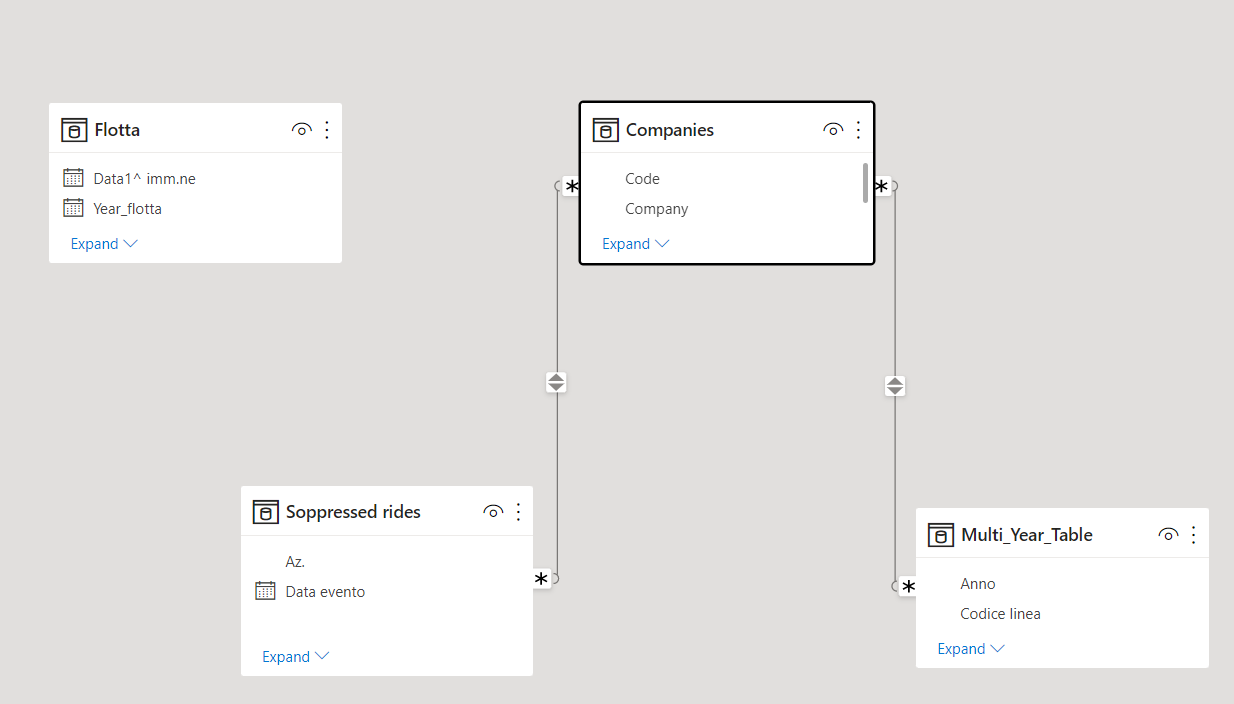
\includegraphics[width=0.9\textwidth]{Images/traditional_dashboard/ER_model.png}
    \caption{ER model of the Dashboard}
    \label{fig:ER}
\end{figure}
\section{Dashboard}

Starting from these tables, a dashboard is designed. It will be divided in subcategories that differ each other for the topic shown. In particular, the themes approached are:
\begin{itemize}
\item Suppressed rides
\item Emissions
\item Operative performances
\item KPIs correlation
\item Economics
\end{itemize}
\subsection{Suppressed rides}
In the following page has been presented the dashboard
\newpage
\begin{landscape}
\thispagestyle{empty}
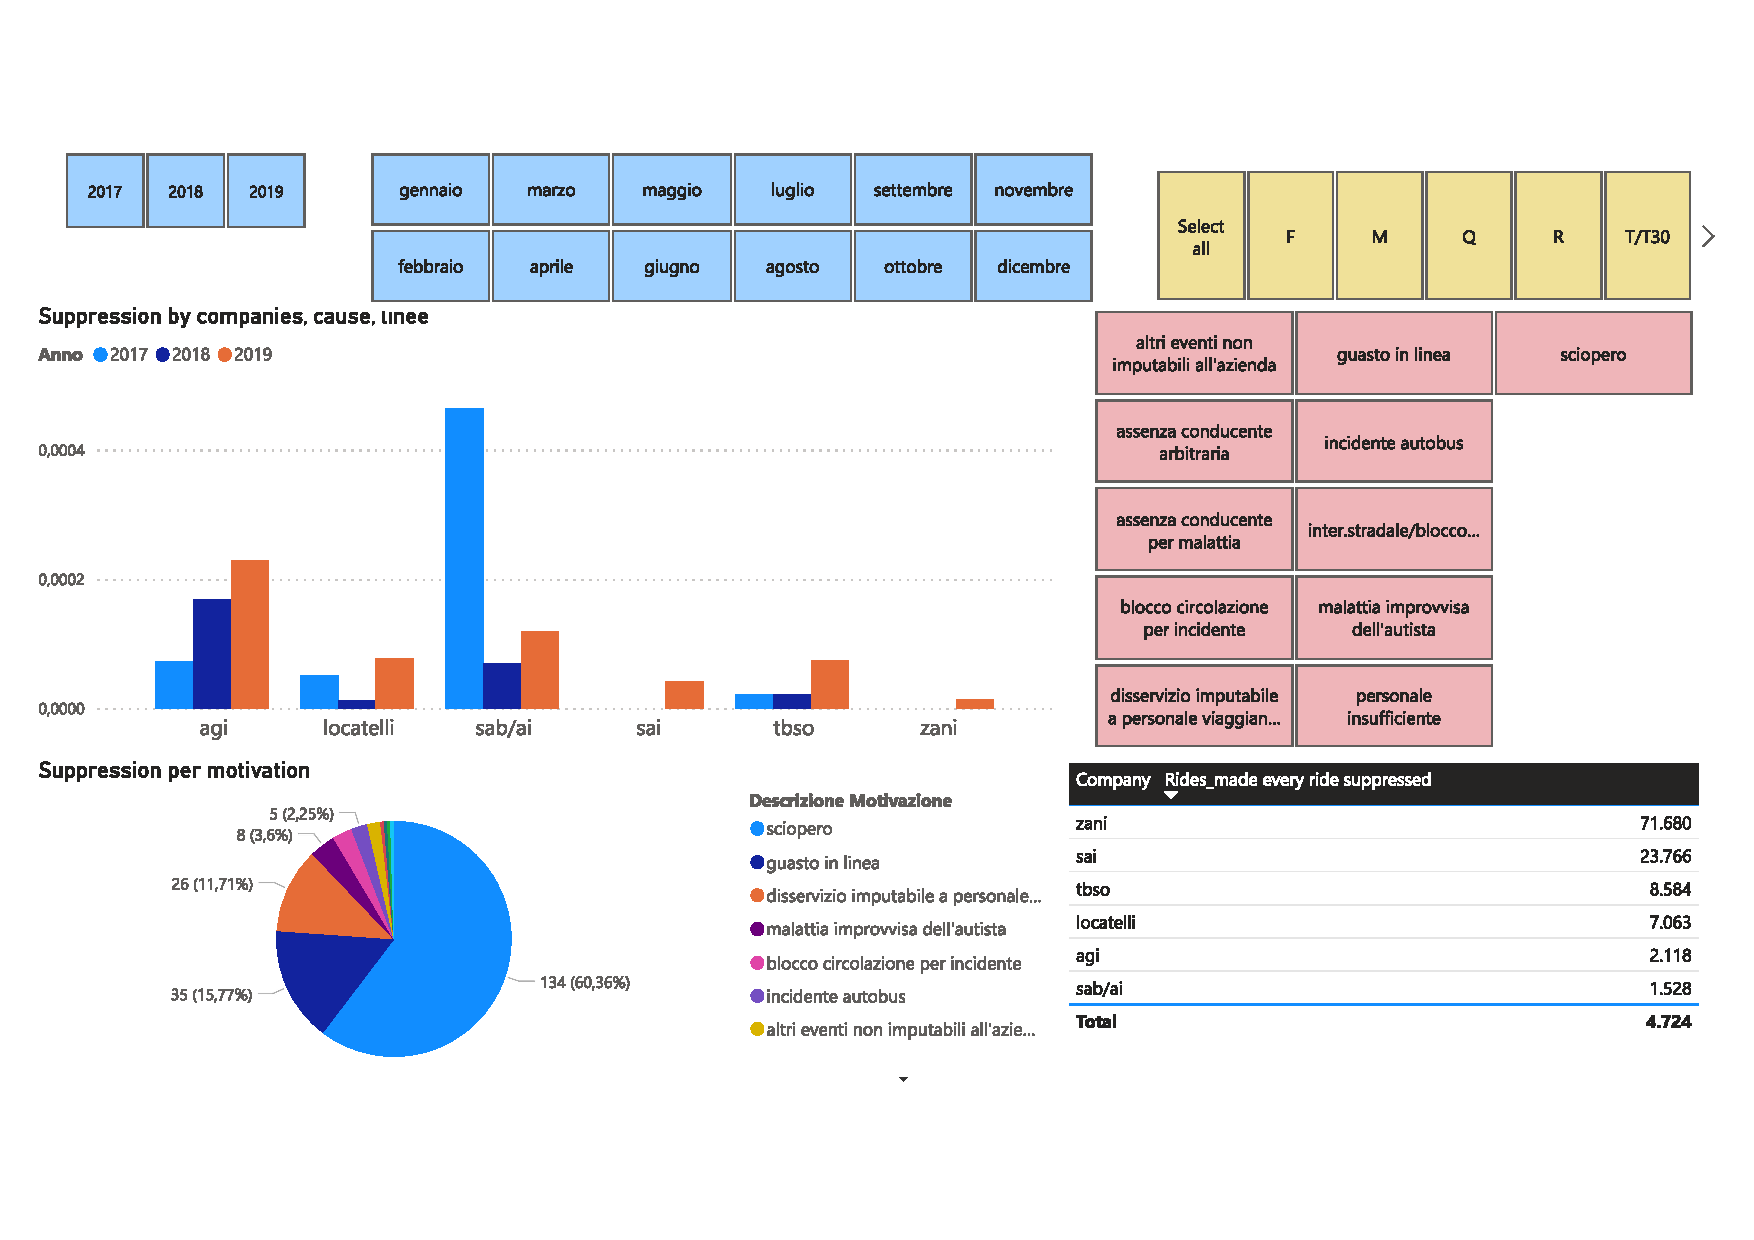
\includepdf[angle=90, pagecommand={\null\enlargethispage{2\baselineskip}\vfill\captionof{figure}{Suppressed}}]{dashboard/Suppression.pdf}
\end{landscape}
\newpage
As said before, data about suppressed rides are between 2017 and 2019. An area of this part of the page is dedicated to filters, thanks to which data can be visualized according to:
\begin{itemize}
\item  period of time with a level of detail equal to a month
\item line
\item reason for which the ride was suppressed
\end{itemize}
Obviously, these filters could be used at the same time in order to obtain very specific analysis.

The table on the bottom right shows the number of rides traveled per each ride suppressed for each company. So, a low number corresponds to a bad result for the company. This data is computed in a relative way in order to show if a company has bad performances according to its dimension. A ride suppressed for a small company is not comparable with few rides suppressed for a big one. 

The pie chart has the goal of showing how the different causes affects suppressed rides, while the histogram shows the total suppressed rides for each year divided by company. 

Considering the dashboard without applying any filter, some considerations can be already done. In 2017 Sab/ai had a huge issue with suppressed rides that reached a percentage level double than the second highest one, in the analyzed period. In 2017 and 2018 Sai and Zani had no problems and their suppressed rides are equal to zero. Finally, Agi had a ever increasing problem related to suppressed rides. 

Moreover, the main cause that brings to a suppressed ride is strike followed at a distance by failure happened during service and inconvenience due to drivers during service. 

Finally, companies with performances below Consortium average are Agi and Sab/ai with, respectively, a ride suppressed every 2,118 and 1,528 rides traveled. 

\newpage

\begin{landscape}
\thispagestyle{empty}
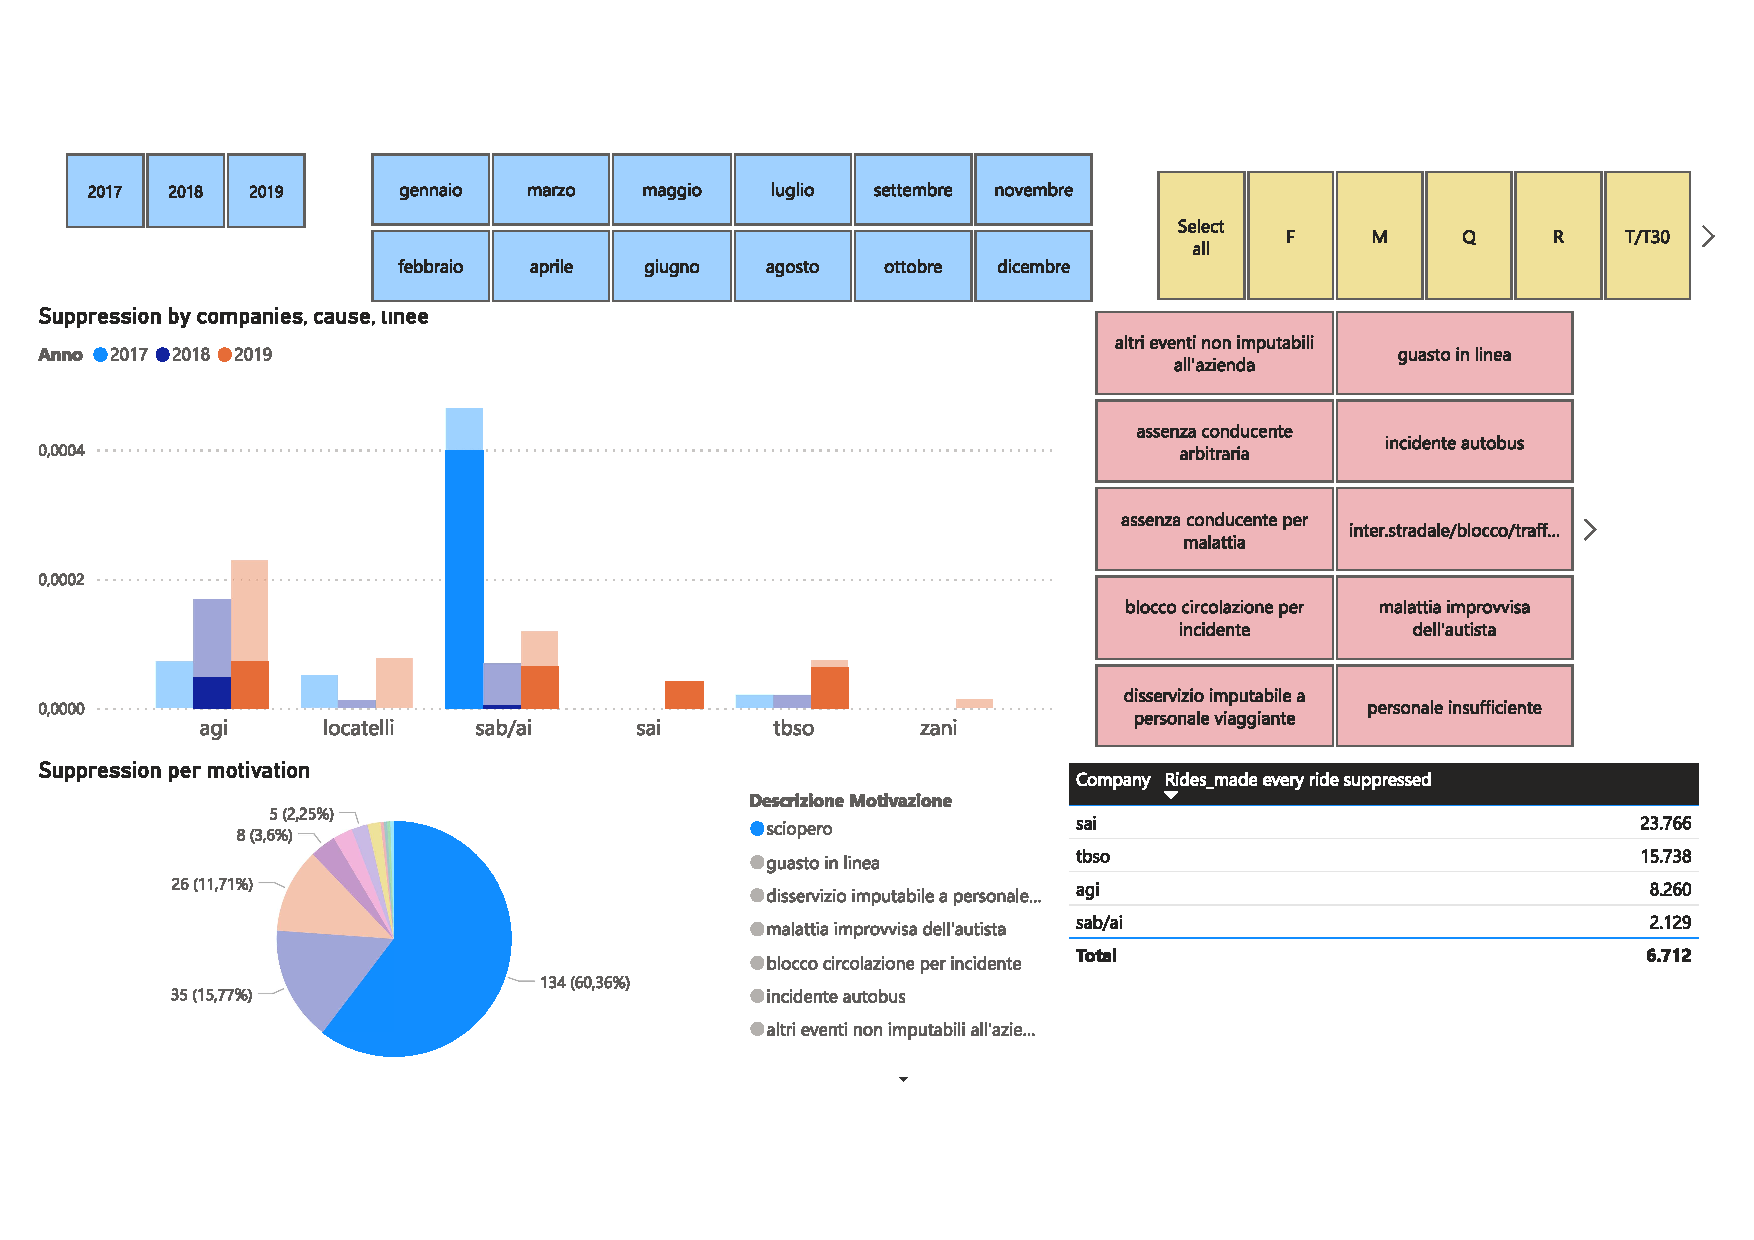
\includepdf[angle=90,  pagecommand={\null\enlargethispage{2\baselineskip}\vfill\captionof{figure}{Suppressed for strikes}\label{fig:strikes}}]{dashboard/Suppression_for_strikes.pdf}
\end{landscape}
\newpage

A focus on the strikes, shown in figure \ref{fig:strikes}, gives several information. Strikes are the reason of the abnormal problems tha Sab/ai had in 2017, moreover a strike in 2019 hit almost every company in an equal measure and, finally, Agi growing issues during this period are reflected also in strikes trend. 

Filtering data according to failure happened during service, a very interesting result is shown: half of the total failures happened during the three year in the Consortium happened during a ride performed by Agi even if Agi is one of the companies with less kilometers run per year. Moreover, this problem in absolute terms remains constant during the year and the negative trend of Agi is due to the increasing of other issues that in 2017 were almost absent.

\newpage
\begin{landscape}
\thispagestyle{empty}
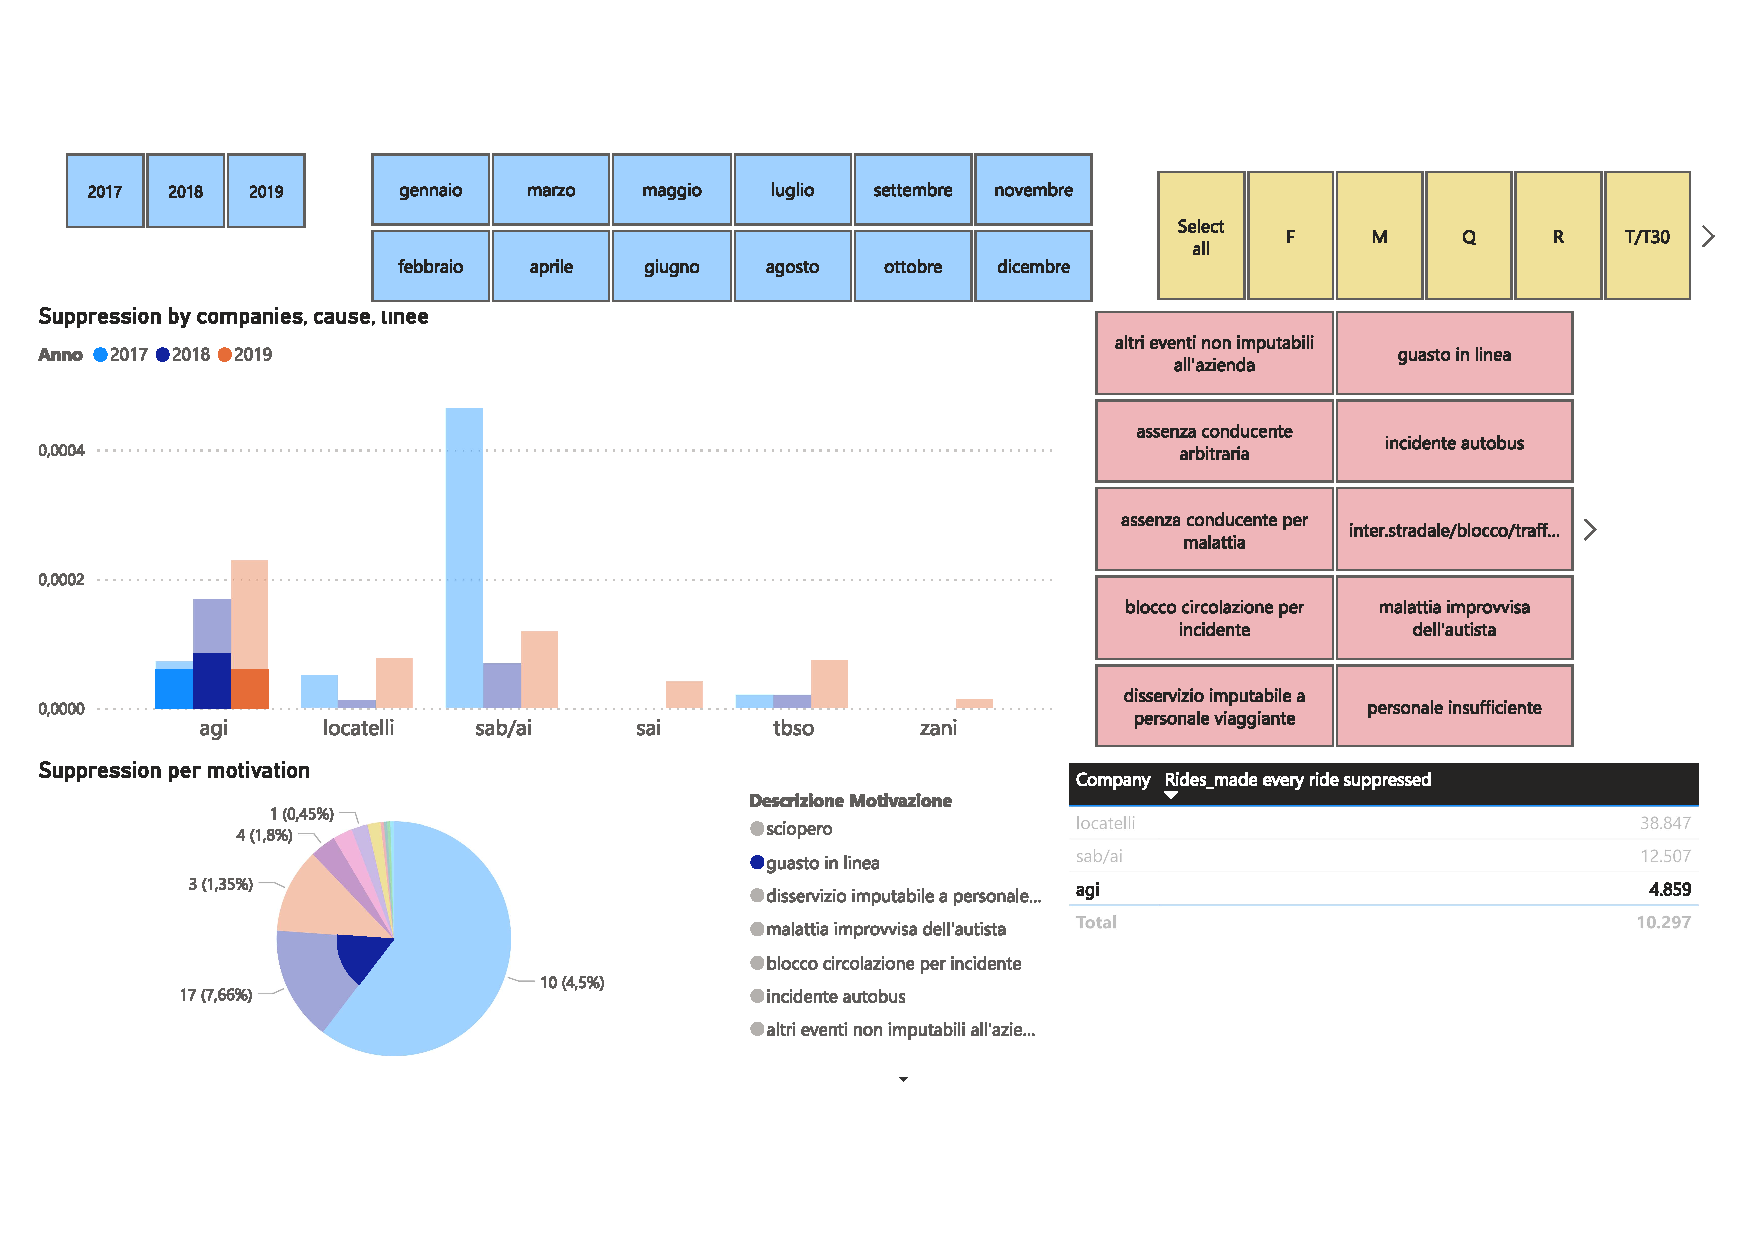
\includepdf[angle=90, pagecommand={\null\enlargethispage{2\baselineskip}\vfill\captionof{figure}{Focus on Agi and fault on the line}\label{fig:failline}}]{dashboard/Suppression_for_fail_on_the_line.pdf}
\end{landscape}
\newpage

\chapter{Innovative KPIs}
\label{ch:Innovative}
\section{Introduction on the Innovative KPIs}
\label{sec:Intro_Innvovative}
In the last few years there is a growing interest in the concept of sustainability and sustainable transportation. New technologies and new objective to be achieved make it necessary to define new indicators to measure the new relevant aspects related to sustainability.

The fundamental role of sustainable development is also confirmed by the 2030 Agenda for Sustainable Development, adopted by all United Nations Member States in 2015. It provides a shared blueprint for peace and prosperity for people and the planet, now and into the future. 

The 2030 Agenda defines \emph{17 Sustainable Development Goals (SDGs)}\cite{sdgs} refer to different areas of social, economic and environmental development and each goal has specific objectives to be achieved over the next few years. 

In the following table the 17 SDGs are reported the ONU target in 2030 and the respective sustainability topics that can be faced in a public transport company.


\newpage
\newpage

\begin{minipage}[c]{0.2\textwidth}
\centering
SDGs ONU
\end{minipage}
\fbox{
\begin{minipage}[c]{0.5\textwidth}
\centering
Target ONU 2030
\end{minipage}
}
\begin{minipage}[c]{0.2\textwidth}
\centering
LPT 
\end{minipage}


\begin{minipage}[c]{0.2\textwidth}
    
\includegraphics[width=\textwidth]{Images/Social_sustainability/1_no_poverty.png}
\end{minipage}
\fbox{
\begin{minipage}[c]{0.5\textwidth}
1.3 Apply at national level adequate systems and social protection measures for all, including minimum levels, and by 2030 achieve substantial coverage of the poor and vulnerable
\end{minipage}
}
\begin{minipage}[c]{0.2\textwidth}
\emph{Corporate welfare}
\end{minipage}


\begin{minipage}[c]{0.2\textwidth}
    
\includegraphics[width=\textwidth]{Images/Social_sustainability/3_helth.png}
\end{minipage}
\fbox{
\begin{minipage}[c]{0.5\textwidth}
3.8 Achieve universal health coverage, including protection from financial risks, access to essential quality health care services and access to safe, effective, quality and affordable essential drugs and vaccines for all
\end{minipage}
}
\begin{minipage}[c]{0.2\textwidth}
\emph{Corporate welfare}
\end{minipage}

\begin{minipage}[c]{0.2\textwidth}
    
\includegraphics[width=\textwidth]{Images/Social_sustainability/white_box.png}
\end{minipage}
\fbox{
\begin{minipage}[c]{0.5\textwidth}
3.6 By 2020, halve the number of deaths and injuries from road traffic accidents worldwide
\end{minipage}
}
\begin{minipage}[c]{0.2\textwidth}
\emph{Health and safety}
\end{minipage}

\begin{minipage}[c]{0.2\textwidth}
    
\includegraphics[width=\textwidth]{Images/Social_sustainability/4_education.png}
\end{minipage}
\fbox{
\begin{minipage}[c]{0.5\textwidth}
4.3 By 2030, ensure equal access for all women and men to affordable, high-quality education, vocational and third-level education, including university

4.4 By 2030, substantially increase the number of young people and adults who have the necessary skills, including technical and professional skills, for employment, decent work and entrepreneurial capacity

4.7 By 2030, ensure that all students acquire the knowledge and skills necessary to promote sustainable development through, inter alia, education for sustainable development and sustainable lifestyles, human rights, equality of gender, the promotion of a culture of peace and non-violence, global citizenship and the enhancement of cultural diversity and the contribution of culture to sustainable development
\end{minipage}
}
\begin{minipage}[c]{0.2\textwidth}
\emph{Training and\\ development}
\end{minipage}
\newpage
\begin{minipage}[c]{0.2\textwidth}
\centering
SDGs ONU
\end{minipage}
\fbox{
\begin{minipage}[c]{0.5\textwidth}
\centering
Target ONU 2030
\end{minipage}
}
\begin{minipage}[c]{0.2\textwidth}
\centering
LPT 
\end{minipage}


\begin{minipage}[c]{0.2\textwidth}
    
\includegraphics[width=\textwidth]{Images/Social_sustainability/5_gender.png}
\end{minipage}
\fbox{
\begin{minipage}[c]{0.5\textwidth}
5.1 End all forms of discrimination against all women, girls and boys
from all over the world

\end{minipage}
}
\begin{minipage}[c]{0.2\textwidth}
\emph{Training and\\ development}
\end{minipage}

\begin{minipage}[c]{0.2\textwidth}
    
\includegraphics[width=\textwidth]{Images/Social_sustainability/white_box.png}
\end{minipage}
\fbox{
\begin{minipage}[c]{0.5\textwidth}
5.5 Guarantee women full and effective participation and equal leadership opportunities at all levels of decision-making in political, economic and public life
\end{minipage}
}
\begin{minipage}[c]{0.2\textwidth}
\emph{Merit\\ management \\of employee}
\end{minipage}

\begin{minipage}[c]{0.2\textwidth}
    
\includegraphics[width=\textwidth]{Images/Social_sustainability/6_water.png}
\end{minipage}
\fbox{
\begin{minipage}[c]{0.5\textwidth}
6.3 By 2030, improve water quality by reducing pollution, eliminating uncontrolled discharge practices and minimizing the release of hazardous chemicals and materials, halve the percentage of untreated wastewater and substantially increase recycling and safe reuse globally

\end{minipage}
}
\begin{minipage}[c]{0.2\textwidth}
\emph{Waste}
\end{minipage}

\begin{minipage}[c]{0.2\textwidth}
    
\includegraphics[width=\textwidth]{Images/Social_sustainability/white_box.png}
\end{minipage}
\fbox{
\begin{minipage}[c]{0.5\textwidth}
6.4 By 2030, substantially increase water efficiency to be used in all sectors and ensure freshwater withdrawals and supplies to address water scarcity and substantially reduce the number of people suffering from water scarcity
\end{minipage}
}
\begin{minipage}[c]{0.2\textwidth}
\emph{Water \\consumption}
\end{minipage}


\begin{minipage}[c]{0.2\textwidth}
    
\includegraphics[width=\textwidth]{Images/Social_sustainability/7_energy.png}
\end{minipage}
\fbox{
\begin{minipage}[c]{0.5\textwidth}
7.2 By 2030, significantly increase the share of renewables in the global energy mix

7.3 By 2030, double the global rate of energy efficiency improvement
\end{minipage}
}
\begin{minipage}[c]{0.2\textwidth}
\emph{Energetic\\ consumption}
\end{minipage}

\newpage

\begin{minipage}[c]{0.2\textwidth}
    
\includegraphics[width=\textwidth]{Images/Social_sustainability/8_work.png}
\end{minipage}
\fbox{
\begin{minipage}[c]{0.5\textwidth}
8.1 Supporting per capita economic growth according to national circumstances and, in particular, at least 7 percent annual growth of gross domestic product in least developed countries
\end{minipage}
}
\begin{minipage}[c]{0.2\textwidth}
\emph{Production and distribution of economic value}
\end{minipage}

\begin{minipage}[c]{0.2\textwidth}
    
\includegraphics[width=\textwidth]{Images/Social_sustainability/white_box.png}
\end{minipage}
\fbox{
\begin{minipage}[c]{0.5\textwidth}
8.2 Achieve higher levels of economic productivity through diversification, technological updating and innovation, including through a focus on high value-added sectors and labour-intensive sectors
\end{minipage}
}
\begin{minipage}[c]{0.2\textwidth}
\emph{Quality of service, customer satisfaction}
\end{minipage}


\begin{minipage}[c]{0.2\textwidth}
    
\includegraphics[width=\textwidth]{Images/Social_sustainability/white_box.png}
\end{minipage}
\fbox{
\begin{minipage}[c]{0.5\textwidth}
8.4 Progressively improve, until 2030, the efficiency of global resources in consumption and production in an attempt to decouple economic growth from environmental degradation, in accordance with the ten-year framework of programs on sustainable consumption and production, with developed countries taking the initiative
\end{minipage}
}
\begin{minipage}[c]{0.2\textwidth}
\emph{Supply-chain management}
\end{minipage}

\begin{minipage}[c]{0.2\textwidth}
    
\includegraphics[width=\textwidth]{Images/Social_sustainability/white_box.png}
\end{minipage}
\fbox{
\begin{minipage}[c]{0.5\textwidth}
8.5 By 2030, achieve full and productive employment and decent work for all women and men, including young people and people with disabilities, and equal pay for work of equal value

8.6 By 2020, substantially reduce the percentage of unemployed young people who do not follow a course of study or who do not follow training courses
\end{minipage}
}
\begin{minipage}[c]{0.2\textwidth}
\emph{Corporate welfare}
\end{minipage}

\begin{minipage}[c]{0.2\textwidth}
    
\includegraphics[width=\textwidth]{Images/Social_sustainability/white_box.png}
\end{minipage}
\fbox{
\begin{minipage}[c]{0.5\textwidth}
8.8 Protect labour rights and promote a safe and secure working environment for all workers, including migrant workers, especially migrant women, and those in precarious work
\end{minipage}
}
\begin{minipage}[c]{0.2\textwidth}
\emph{Health and safety of workers}
\end{minipage}

\newpage

\begin{minipage}[c]{0.2\textwidth}
    
\includegraphics[width=\textwidth]{Images/Social_sustainability/9_industry.png}
\end{minipage}
\fbox{
\begin{minipage}[c]{0.5\textwidth}
9.1 Develop quality, reliable, sustainable and resilient infrastructure, including regional and cross-border infrastructure, to support economic development and human well-being, with a focus on equitable access for all
\end{minipage}
}
\begin{minipage}[c]{0.2\textwidth}
\emph{Quality of service, accessibility, customer satisfaction}
\end{minipage}

\begin{minipage}[c]{0.2\textwidth}
    
\includegraphics[width=\textwidth]{Images/Social_sustainability/white_box.png}
\end{minipage}
\fbox{
\begin{minipage}[c]{0.5\textwidth}
9.5 Strengthen scientific research, promote the technological capacities of industrial sectors in all countries, in particular in developing countries, including by encouraging innovation by 2030 and by substantially increasing the number of workers in the research and development every million people and public and private spending on research and development
\end{minipage}
}
\begin{minipage}[c]{0.2\textwidth}
\emph{Innovation}
\end{minipage}

\begin{minipage}[c]{0.2\textwidth}
    
\includegraphics[width=\textwidth]{Images/Social_sustainability/white_box.png}
\end{minipage}
\fbox{
\begin{minipage}[c]{0.5\textwidth}
9.6 Significantly increase access to information and communication technologies and strive to provide universal and low-cost access to the Internet in least developed countries by 2020
\end{minipage}
}
\begin{minipage}[c]{0.2\textwidth}
\emph{Digital transformation}
\end{minipage}

\begin{minipage}[c]{0.2\textwidth}
    
\includegraphics[width=\textwidth]{Images/Social_sustainability/10_ineq.png}
\end{minipage}
\fbox{
\begin{minipage}[c]{0.5\textwidth}
10.3 Ensure equal opportunities for all and reduce result inequalities, including through the elimination of discriminatory laws, policies and practices, and the promotion of adequate laws, policies and actions in this regard

10.4 Adopt policies, in particular fiscal, wage and social protection policies, and progressively achieve greater equality
\end{minipage}
}
\begin{minipage}[c]{0.2\textwidth}
\emph{Evaluation, remuneration and incentive system}
\end{minipage}

\newpage
\begin{minipage}[c]{0.2\textwidth}
    
\includegraphics[width=\textwidth]{Images/Social_sustainability/11_cities.png}
\end{minipage}
\fbox{
\begin{minipage}[c]{0.5\textwidth}
11.2 By 2030, provide access to safe, sustainable, and affordable transport systems for all, improve road safety, in particular by expanding public transport, with particular attention to the needs of those in vulnerable situations, women, children, people with disabilities and the elderly
\end{minipage}
}
\begin{minipage}[c]{0.2\textwidth}
\emph{Accessibility of service}
\end{minipage}

\begin{minipage}[c]{0.2\textwidth}
    
\includegraphics[width=\textwidth]{Images/Social_sustainability/white_box.png}
\end{minipage}
\fbox{
\begin{minipage}[c]{0.5\textwidth}
11.3 By 2030, increase inclusive and sustainable urbanization and the capacity for participatory and integrated planning and management of human settlement in all countries
\end{minipage}
}
\begin{minipage}[c]{0.2\textwidth}
\emph{Community}
\end{minipage}

\begin{minipage}[c]{0.2\textwidth}
    
\includegraphics[width=\textwidth]{Images/Social_sustainability/white_box.png}
\end{minipage}
\fbox{
\begin{minipage}[c]{0.5\textwidth}
11.6 By 2030, reduce the negative per capita environmental impact of cities, in particular with regard to air quality and waste management
\end{minipage}
}
\begin{minipage}[c]{0.2\textwidth}
\emph{Emissions}
\end{minipage}

\begin{minipage}[c]{0.2\textwidth}
    
\includegraphics[width=\textwidth]{Images/Social_sustainability/12_consumption.png}
\end{minipage}
\fbox{
\begin{minipage}[c]{0.5\textwidth}
12.2 By 2030, achieve sustainable management and efficient use of natural resources
\end{minipage}
}
\begin{minipage}[c]{0.2\textwidth}
\emph{Consumption of energy and natural resources, waste management}
\end{minipage}

\begin{minipage}[c]{0.2\textwidth}
    
\includegraphics[width=\textwidth]{Images/Social_sustainability/white_box.png}
\end{minipage}
\fbox{
\begin{minipage}[c]{0.5\textwidth}
12.6 Encourage businesses, especially large and transnational companies, to adopt sustainable practices and integrate sustainability information into their reporting
\end{minipage}
}
\begin{minipage}[c]{0.2\textwidth}
\emph{Governance of sustainability and supply chain}
\end{minipage}

\begin{minipage}[c]{0.2\textwidth}
    
\includegraphics[width=\textwidth]{Images/Social_sustainability/13_climate.png}
\end{minipage}
\fbox{
\begin{minipage}[c]{0.5\textwidth}
13.2 Integrate measures to combat climate change into national policies, strategies and plans
\end{minipage}
}
\begin{minipage}[c]{0.2\textwidth}
\emph{Emission of GHG}
\end{minipage}

\begin{minipage}[c]{0.2\textwidth}
    
\includegraphics[width=\textwidth]{Images/Social_sustainability/16_peace.png}
\end{minipage}
\fbox{
\begin{minipage}[c]{0.5\textwidth}
16.5 Substantially reduce corruption and all its forms

16.4 By 2030, significantly reduce illicit financing and arms trafficking, enhance the recovery and return of stolen assets and fight all forms of organized crime
\end{minipage}
}
\begin{minipage}[c]{0.2\textwidth}
\emph{Community}
\end{minipage}

\begin{minipage}[c]{0.2\textwidth}
    
\includegraphics[width=\textwidth]{Images/Social_sustainability/white_box.png}
\end{minipage}
\fbox{
\begin{minipage}[c]{0.5\textwidth}
16.6 Develop effective, accountable and transparent institutions at all levels
\end{minipage}
}
\begin{minipage}[c]{0.2\textwidth}
\emph{Production and distribution of economic value}
\end{minipage}

\begin{minipage}[c]{0.2\textwidth}
    
\includegraphics[width=\textwidth]{Images/Social_sustainability/white_box.png}
\end{minipage}
\fbox{
\begin{minipage}[c]{0.5\textwidth}
16.7 Ensure responsive, inclusive, participatory and representative decision making at all levels
\end{minipage}
}
\begin{minipage}[c]{0.2\textwidth}
\emph{Customer satisfaction and community attention}
\end{minipage}

\begin{minipage}[c]{0.2\textwidth}
    
\includegraphics[width=\textwidth]{Images/Social_sustainability/white_box.png}
\end{minipage}
\fbox{
\begin{minipage}[c]{0.5\textwidth}
16.8 Promote and enforce non-discriminatory laws and policies for sustainable development
\end{minipage}
}
\begin{minipage}[c]{0.2\textwidth}
\emph{Ethics}
\end{minipage}

\newpage

\begin{minipage}[c]{0.2\textwidth}
    
\includegraphics[width=\textwidth]{Images/Social_sustainability/17_partnerships.png}
\end{minipage}
\fbox{
\begin{minipage}[c]{0.5\textwidth}
17.13 Enhance global macro-economic stability, including through policy coordination and coherence

17.14 Improve policy coherence for sustainable development
\end{minipage}
}
\begin{minipage}[c]{0.2\textwidth}
\emph{Community attention}
\end{minipage}

\begin{minipage}[c]{0.2\textwidth}
    
\includegraphics[width=\textwidth]{Images/Social_sustainability/white_box.png}
\end{minipage}
\fbox{
\begin{minipage}[c]{0.5\textwidth}
17.19 By 2030, build, on the basis of existing initiatives, systems for measuring progress towards sustainable development that are complementary to measuring GDP and support the creation of statistical capacity in developing countries

17.17 Encourage and promote effective partnerships in the public sector, between public and private and in civil society based on the experience of partnerships and their ability to find resources
\end{minipage}
}
\begin{minipage}[c]{0.2\textwidth}
\emph{Governance of sustainability}
\end{minipage}


\newpage

In order to better analyse these new aspects, the EU directive 2014/95\cite{directive201495eu} establishes that public interest companies, that meet a number of requirements, are required to provide a non-financial report. This annual sustainability report makes it possible to communicate the performance and sustainability impacts of a company. It consists of measuring, communicating and assuming responsibility towards stakeholders in relation to the performance of the organization with respect to the goal of sustainable development. The topic addressed in this report are:

\begin{itemize}
    \item Environmental topic
    \item Social and diversity equality topic
    \item Respect for human rights
    \item Anti-corruption and extortion
\end{itemize}

Given the importance of these new topics, the next paragraphs will be dedicated to identifying new indicators related to these new aspects. In particular, the \ref{sec:newtech} identifies the new technologies already on the market and other new technologies that are still in the research phase, but which will become more relevant in the future. Subsequently it is shown how new technologies and new data collected can lead to the definition of new indicators for green sustainability, social sustainability and maintenance.

Before identifying these new KPIs, it is good to remember the \emph{characteristics of a good indicator}.

First, indicators are measured to evaluate progress and they can be defined in terms of goals, objectives, targets and thresholds. For example, a planning process may involve establishing traffic congestion indicators (defining how congestion will be measured), goals (a desire for fast and efficient vehicle travel), objectives (changes in roadway supply or travel activity that reduces congestion) and targets (specific, feasible changes in congestion impacts or travel behavior that should be achieved), and thresholds (levels beyond which additional actions will be taken to reduce congestion).

Indicators can reflect various levels of analysis. For example, indicators may reflect the decision-making process (quality of planning), responses (travel patterns), physical impacts (emission and crash rates), human and environmental effects (injuries and deaths, and ecological damages), and their economic impacts (costs of crash and environmental damages).

Another way to classify the indicators in the following:
\begin{itemize}
    \item \emph{Process} the types of policies and planning activities, such as whether the organization has a process for collecting and publishing performance data, and public involvement.
    \item \emph{Inputs} the resources that are invested activities, such as the level of funding spent on various activities or modes.
    \item \emph{Outputs} direct results, such as the miles of sidewalks, paths and roads, and the amount of public transit service provided.
    \item \emph{Outcomes} ultimate results, such as the number of miles traveled and mode share, average travel speeds, congestion and crowding, number of accidents and casualties, energy consumption, pollution emissions, and user satisfaction.
\end{itemize}
It is often best to use some of each type of performance indicators. 

Another aspect to consider is the use of qualitative or quantitative data. Quantitative data refers to easy-to-measure information, while qualitative data refers to other types of information and they can be quantified using letter or number ratings. 

Relative indicators are often used to evaluate many impacts, such as trends or comparisons with peers. Reference units (also called ratio indicators) are measurement units normalized to facilitate comparisons, such as per-year, per-capita, per-mile, per-trip, per-vehicle-year and per dollar. The selection of reference units can affect how problems are defined and solutions prioritized. For example, measuring impacts such as emissions, crashes and costs per vehicle-mile ignores the effects of changes in vehicle mileage. Measuring these impacts per capita does account for changes in vehicle travel.

Summing up the \emph{principles to consider selecting a new KPI} are:
\begin{itemize}
    \item Relevance to the community's definition of sustainability, considering the suburban or urban area
    \item Understandability by the community at large, not only experts
    \item Acceptance and usage by the community
    \item Long-term view of the community
    \item Integration of different relevant topic
    \item Based on information that is reliable, accessible, timely and accurate
    \item Consideration of local impacts at the expense of global impacts
    \item Quantitative KPIs are easier to analyse, they are considered more objective and they tends to receive more weight in a planning process. Sustainability indicators therefore require quantifying impacts as much as possible.
    \item trade-off between smaller set of indicators, using available data, and larger set can be more comprehensive but have excessive data collection and analysis costs. 
\end{itemize}


\chapter{Innovative KPI}

From sustainability balance sheets
From new technologies installed on buses now and in the next future



%-------------------------------------------------------------------------
%	BIBLIOGRAPHY
%-------------------------------------------------------------------------

\addtocontents{toc}{\vspace{2em}} % Add a gap in the Contents, for aesthetics
\bibliography{references} % The references information are stored in the file named "Thesis_bibliography.bib"
\nocite{*}

%-------------------------------------------------------------------------
%	APPENDICES
%-------------------------------------------------------------------------

%\cleardoublepage
%\addtocontents{toc}{\vspace{2em}} % Add a gap in the Contents, for aesthetics
%\appendix
%\chapter{Appendix A}

% LIST OF FIGURES
\listoffigures

% LIST OF TABLES
\listoftables

% LIST OF SYMBOLS
% Write out the List of Symbols in this page


% ACKNOWLEDGEMENTS
%\chapter*{Acknowledgements}
%Here you might want to acknowledge someone.

%\cleardoublepage

\end{document}
